% Cover letter using letter.sty

\documentclass[11pt]{letter} % Uses 10pt
\usepackage{graphicx,subfigure}
\usepackage{float}
\usepackage{caption}
\captionsetup{labelsep=space}

\renewcommand*{\figureformat}{\figurename~\thefigure}

\restylefloat{figure}
%Use \documentstyle[newcent]{letter} for New Century Schoolbook postscript font
% the following commands control the margins:
\topmargin=-1.2in    % Make letterhead start about 1 inch from top of page 
\textheight=14in  % text height can be bigger for a longer letter
\oddsidemargin=0pt % leftmargin is 1 inch
\textwidth=6.5in   % textwidth of 6.5in leaves 1 inch for right margin
\textheight 255mm


\begin{document}\pagenumbering{gobble}




\begin{flushleft}
{\large\bf Eamon O'Gorman}
\end{flushleft}
\medskip\hrule height 1pt
\begin{flushright}


\end{flushright} 
%\vfill % forces letterhead to top of page
{\Large 
\begin{center}
Understanding the Mechanisms which Drive the Winds of Red Giants and Red Supergiants
\end{center}
}

My main research interests lie in understanding the dynamics and thermodynamics of the atmospheres of red giants (pre-asymptotic giant branch red giants) and red supergiants (RSGs), through both modelling and observational techniques. The mass-loss from these stars plays a crucial role in galactic evolution and ultimately provides much of the material required for the next generation of stars and planets. This mass-loss occurs via a cool ($T_{e} \leq 10^4\,K$) wind, with terminal velocities ($10 \leq v_{\infty} \leq 50$\,km\,s$^{-1}$) typically less than the photospheric escape velocity ($v_{\rm{esc}} \sim 100$\,km\,s$^{-1}$). A substantial fraction of the star's initial mass can be dispersed to the interstellar medium during these post main sequence evolutionary stages and this mass-loss is therefore a crucial factor governing stellar evolution, and also in explaining the frequency of supernovae in the galaxy. Despite the importance of this phenomenon, and decades of study, the specific mechanisms that drive winds from evolved spectral-type K through mid-M stars remain unknown. There is insufficient atomic, molecular, or dust opacity to drive a radiation-driven outflow and acoustic/pulsation models cannot drive the observed mass-loss rates. UV and optical observations reveal an absence of significant hot wind plasma, and the winds are thus too cool to be Parker-type thermally-driven flows. Magnetic fields are most likely involved in the mass-loss process, although current magnetic models are also unable to explain spectral diagnostics. Traditionally, observations have provided only limited disk-averaged information about the outflow environments of these stars, making it difficult to infer the outflow properties. However, the latest suite of interferometers now have the capability to provide essential spatial information on these outflow environments.

Betelgeuse is one of the few nearby RSGs that can be studied in great detail across most of the electromagnetic spectrum. The extended atmosphere of this oxygen-rich RSG provides an ideal testbed for studying the poorly understood processes that drive mass-loss from K and M supergiants. Part of my research to date has focused on explaining and reconciling the puzzling results from previous single dish millimeter observations of this star's circumstellar environment. Ro-vibrational absorption lines of $^{12}$C$^{16}$O and $^{13}$C$^{16}$O by Bernat et al. (1979) revealed that Betelgeuse has undergone at least two distinct phases of mass-loss in its recent past. However, previous millimeter observations were only able to detect one component of the outflow, while the spatial extent of both components were unknown. Using multiple array configurations of the CARMA interferometer, we successfully imaged the CO($J = 2 - 1$) emission line at sub-arcsecond resolution, and for the first time were able to find the spatial extent of both outflow components, allowing their ages to be calculated. We also found both components to be inhomogeneous, far from the existing spherically symmetric models of its circumstellar environment, indicating a chaotic mass-loss loss process. I am part of a collaboration that has been awarded ALMA cycle 1 time (PI: P. Kervella) which will trace CO emission around Betelgeuse at a resolution 10 times better than we achieved with CARMA. This project will also provide insight into the role dust plays in the mass-loss of Betelgeuse, a relatively non-dusty M supergiant.

In the 1980's, heating and acceleration by magnetic waves appeared to be a promising explanation for driving mass-loss in RSGs, but spatially resolved VLA cm-continuum radio maps (Lim et al. 1996) revealed that Betelgeuse's extended atmosphere ($2-7\,R_{\star}$) was significantly cooler and much less ionized than predicted. I have been involved in a collaboration which used e-MERLIN to image the thermal continuum emission from this inner region of Betelgeuse's atmosphere at 6\,cm. We have discovered two ``chromospheric hotspots'' (Figure 1, \textit{left}) separated by $4\,R_{\star}$, hidden just beyond the spatial resolution of the VLA at 6\,cm. Using the astrometric solution of Harper et al. (2008), I have shown that the brighter feature ($T_{e} > 5400$,\K) is $\sim 3.5\,R_{\star}$ from the photosphere. Inspired by this new discovery, I am currently undertaking a study of multi-wavelength multi-epoch centimeter VLA data which contains the Pie Town VLBA antenna. At the highest available frequencies, these data have even superior spatial resolution than e-MERLIN (at 6\,cm) and the idea is to look for signatures of these hotspots. In Figure 1 (right) a preliminary map at 0.7\,cm is presented, and evidence of at least two features separated by only $2\,R_{\star}$ is shown. These features may be generated by  giant photospheric convective cells, although it is unlikely that such features could be accountable for the ``hotspots'' seen with e-MERLIN. Frequent multi-wavelength high spatial resolution monitoring of Betelgeuse with e-MERLIN is required to solve this puzzling evidence and this project would be one of my main priorities in my first year as an ESO fellow.

I have recently used the Karl G. Jansky Very Large Array to observe two non-dusty, non-pulsating, K spectral-type red giants at multiple radio wavelengths ($0.7 - 20$\,cm). The nature of free-free radio opacity allowed us to probe different layers of their atmospheres, and we found evidence for a rapidly cooling stellar wind for one of the targets. We also found that our observations were in disagreement with the existing atmospheric models for these stars, which were based on UV diagnostics. Another aim as an ESO fellow would be to create new atmospheric models for these stars, which would be based on this new VLA data and also on millimeter CARMA data (which also needs to be reduced). These data are sensitive to over four orders of magnitude in continuum optical depth, and our hydrogen ionization code which I am developing would provide the most detailed atmospheric models of such stars to date. Such models can then be used to carry out detailed thermal energy balances allowing potential mass-loss mechanisms to be investigated.

I am also leading a project to detect radio emission from $\beta$ Gem b, an exoplanet orbiting the closet red giant, Pollux. Previous searches for exoplanet radio emission have focused on close orbiting planets, the so-called \textit{hot Jupiters}. Our target is further away from its host star and probable free from tidal locking, which may reduce the internal magnetic field of the hot Jupiters, thus reducing the strength of the radio emission. We expect the relatively large mass-loss of the host red giant to be a key driver in detecting this emission. We are currently using the GMRT to search for this emission at 150\,MHz, and I also plan to carry out observations at lower frequencies with LOFAR.

The latest suite of radio and millimeter interferometers are now allowing exciting new research to be carried out on evolved stars and an ESO fellowship would enable me to to continue with this research. Collaborations
make the strongest interpretation of science and my research interests also overlap and complement those of the stellar structure and evolution group at ESO-Garching.

\begin{figure}[!ht]
\centering 
\mbox{
          \includegraphics[trim=27pt 90pt 40pt 90pt,clip,angle=90,width=8cm,height=7cm]{/home/eamon/Documents/eso/plan/fig1.ps}
          \includegraphics[trim=145pt 587pt 140pt 20pt,clip,width=9.5cm,height=7.0cm]{/home/eamon/Documents/eso/plan/fig0.ps}
          }
\caption{ {\small  \textbf{Figure 1.} \textit{Left:} e-MERLIN 6\,cm image of Betelgeuse showing the two chromospheric ``hotspots''. The red filled circle marks the expected photospheric position. \textit{Right:} VLA + Pie Town 0.7\,cm image of Betelgeuse's inner asymmetric atmosphere. The presence of giant photospheric convective cells can account for the asymmetries in the 0.7\,cm image, but cannot account for the hotspot at $\sim 3.5\,R_{\star}$ in the 6\,cm image.}}
\end{figure}




\end{flushright}
\end{document}






